En este cap�tulo se realizo el dise�o del controlador PID a utilizar por el m�todo de asignaci�n de polos, con el calculo de los par�metros para  planta estudiada en el cap�tulo \ref{CAP:accio} y la interfaz para ajustar los valores de $k_{p}$, $k_{i}$ y $k_{d}$ del controlador para plantas de segundo orden.  

\section{Pasos para el dise�o del controlador.}

Se dise�� un controlador PID con el m�todo de asignaci�n de polos, en el cu�l se tienen las siguientes consideraciones para realizarlo:

\begin{itemize}
	\item Un sistema de segundo orden descrito por la ecuaci�n \ref{ec:segundoorden}
	\begin{center}
		$
			F(s)=\dfrac{K\omega_{n}^{2}}{s^{2}+2\zeta \omega_{n}s+\omega_{n}^{2}}
		$
	\end{center} 

\item La ecuaci�n del controlador PID en paralelo como se muestra en el diagrama de bloques de la figura \ref{fig:controlpa} y la ecuaci�n viene dada por \ref{ec:contro}

 \begin{figure}[H]
	\centering
	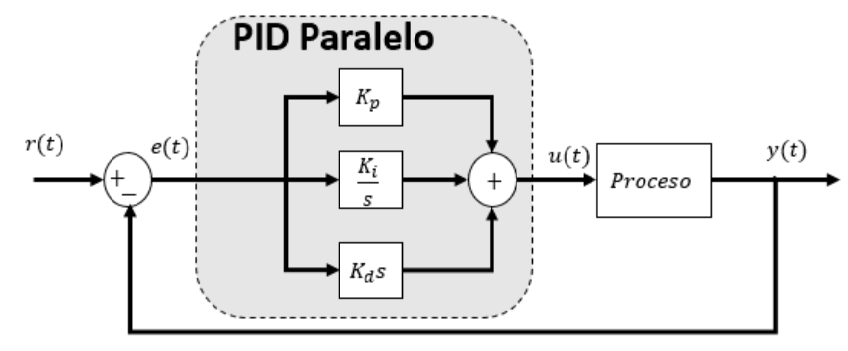
\includegraphics[scale=0.7]{img/controlpa}
	\caption{Sistema de control en lazo cerrado con control PID.}
	\label{fig:controlpa}
\end{figure}


\begin{center}
	\begin{equation}\label{ec:contro}
		C(s)=K_{p}+K_{d}s+\dfrac{K_{i}}{s}=\frac{K_{d}s^{2}+K_{p}s+K_{i}}{s}
	\end{equation}
\end{center}

Donde:
\begin{itemize}
	\item  $K_{p}$= Es la ganancia proporcional.
	\item $K_{i}$= Es la ganancia integral del controlador.
	\item $K_{d}$= Es la ganancia derivativa del controlador.
\end{itemize}

\item Se le asignan tanto al controlador como al sistema a controlar,coeficientes que representar�n polinomios. 



\begin{center}
	$f(s)=\dfrac{\omega_{n}^{2}}{s^{2}+2\zeta \omega_{n}s+\omega_{n}^{2}}=\frac{K}{s^{2}+as+b}=\dfrac{A}{B}$
\end{center}
 \begin{center}
 	
 	$C(s)=\frac{K_{d}s^{2}+K_{p}s+K_{i}}{s}$=$\dfrac{D}{E}$
 	
 \end{center}

\item La funci�n a lazo cerrado es 
\begin{center}
	$H(s)=\frac{DA}{EB+DA}$
\end{center}

\item Si se reemplaza la ecuaci�n 

\begin{center}
	$H(s)=\frac{K(d_{2}s^{2}+d_{1}s+d_{0})}{s(s^2+as+b)+(d_{2}s^2+d_{1}s+d_{0})K}$
\end{center}

\begin{center}
	\begin{equation}\label{ec:controlfinal}
		H(s)=\frac{Kd_{2}s^{2}+Kd_{1}s+Kd_{0}}{s^{3}+(a+Kd_{2})s^{2}+(b+Kd_{1})s+Kd_{0}}
	\end{equation}
\end{center}

\item Se obtiene una funci�n de transferencia de tercer orden, con dos polos dominantes que son los que rigen la din�mica del sistema. Por este motivo, se debe completar la ecuaci�n caracter�stica que representa al polinomio deseado con otro polo alejado del eje imaginario y de los polos dominantes. Esto con el objetivo de tener un polo que no afecte el comportamiento de los polos dominantes.

Al polo deseado  calculado en \ref{ec:polo}, se le agrega un tercer polo siendo la ecuaci�n general:

\begin{center}
	$P_{d}(s)=(s^{2}+h_{1}s+h_{2})(s+p_{1})$=$s^{3}+\alpha_{1}s^{2}+\alpha_{2}s+\alpha_{3}$
\end{center}

\begin{center}
	$P_{s}(d)=(s^{2}+2.25\cdot 10^{2}s+2.58 \cdot10^{4})(s+1200)=s^{3}+1.42\cdot10^{3}s^{2}+2.95\cdot10^{5}s+30.91\cdot10^{6}$
\end{center}

\item A continuaci�n se igualan las dos ecuaciones caracter�sticas de H(s) y de $P_{s}$, para poder determinar los valores de $ K_{p}$,$ K_{d}$ y $K_{i}$.

\begin{center}
	$s^{3}+(a+Kd_{2})s^{2}+(b+Kd_{1})s+Kd_{0}=s^{3}+\alpha_{1}s^{2}+\alpha_{2}s+\alpha_{3} $
\end{center}

\item Igualando los coeficientes

\subitem $a+Kd_{2}=\alpha_{1}$ 
\subitem $b+Kd_{1}=\alpha_{2}$
\subitem $Kd_{0}=\alpha_{3}$

\item Reemplazando y resolviendo los valores $K_{p}$,$ K_{i}$, $ K_{d}$:


\subitem $K_{d}=\frac{\alpha_{1}-a}{K}$
\subitem $K_{p}=\frac{\alpha_{2}-b}{K}$
\subitem $K_{i}=\frac{\alpha_{3}}{K}$

\item Los valores n�mericos de $K_{p}$,$ K_{i}$, $ K_{d}$: 

\begin{equation}\label{ec:kp}
	K_{p}=\frac{2.95\cdot10^{5}-1.43\cdot10^{5}}{1.43\cdot10^{5}}=1.06
\end{equation}

\begin{equation}\label{ec:ki}
	K_{i}=\frac{30.91\cdot10^{6}}{1.43\cdot10^{5}}=215.7
\end{equation}

\begin{equation}\label{ec:kd}
	K_{d}=\frac{1.42\cdot10^{3}-1.29\cdot10^{4}}{1.43\cdot10^{5}}=-0.08
\end{equation}


\end{itemize}


\section{Controlador.}

En \ref{ec:contro} donde se muestra la ecuaci�n del controlador y a partir de all� se realizaran las ecuaciones de las aproximaciones de las derivadas por definici�n de primer y segundo orden se basan en:

\begin{equation}\label{ec:derivada1}
	sf=\frac{f(t)-f(t-T)}{T}
\end{equation}


\begin{equation}
	s^{2}f=\frac{f'(t)-f'(t-T)}{T}=\frac{\frac{f(t)-f(t-1)}{T}-\frac{f(t-1)-f(t-2)}{T}}{T}=\frac{f(t)-2f(t-1)+f(t-2)}{T^{2}}
\end{equation}

Se tomar� que el valor de T menor a 1, para sacar las muestras en base del periodo el cual permite aproximar la derivada a las expresiones en diferencias mostradas en la las ecuaciones \ref{ec:derivada1} y \ref{ec:segundoordfinal}.



  